% Copyright 2004 by Till Tantau <tantau@users.sourceforge.net>.
%
% In principle, this file can be redistributed and/or modified under
% the terms of the GNU Public License, version 2.
%
% However, this file is supposed to be a template to be modified
% for your own needs. For this reason, if you use this file as a
% template and not specifically distribute it as part of a another
% package/program, I grant the extra permission to freely copy and
% modify this file as you see fit and even to delete this copyright
% notice. 

\documentclass{beamer}

\usepackage[spanish]{babel} % Spanish language/hyphenation
\selectlanguage{spanish}
\usepackage[utf8]{inputenc}
\usepackage{hyperref}

% There are many different themes available for Beamer. A comprehensive
% list with examples is given here:
% http://deic.uab.es/~iblanes/beamer_gallery/index_by_theme.html
% You can uncomment the themes below if you would like to use a different
% one:
%\usetheme{AnnArbor}
%\usetheme{Antibes}
%\usetheme{Bergen}
%\usetheme{Berkeley}
%\usetheme{Berlin}
%\usetheme{Boadilla}
%\usetheme{boxes}
%\usetheme{CambridgeUS}
%\usetheme{Copenhagen}
%\usetheme{Darmstadt}
%\usetheme{default}
%\usetheme{Frankfurt}
%\usetheme{Goettingen}
%\usetheme{Hannover}
%\usetheme{Ilmenau}
%\usetheme{JuanLesPins}
%\usetheme{Luebeck}
\usetheme{Madrid}
%\usetheme{Malmoe}
%\usetheme{Marburg}
%\usetheme{Montpellier}
%\usetheme{PaloAlto}
%\usetheme{Pittsburgh}
%\usetheme{Rochester}
%\usetheme{Singapore}
%\usetheme{Szeged}
%\usetheme{Warsaw}

\title{Robot Motion Planning: A Distributed Representation Approach}

% A subtitle is optional and this may be deleted
\subtitle{Planificación de Tareas y Movimientos de Robots}

\author{Jorge Camarero Vera - 07052\\ Rodrigo Orellana Ferrufino - M15139\\ Kunshen Zhang - M15148}
% - Give the names in the same order as the appear in the paper.
% - Use the \inst{?} command only if the authors have different
%   affiliation.

\institute[] % (optional, but mostly needed)
{
  Máster en Automática y Robótica\\
  Universidad Politécnica de Madrid
}
% - Use the \inst command only if there are several affiliations.
% - Keep it simple, no one is interested in your street address.

\date{Diciembre, 2015}
% - Either use conference name or its abbreviation.
% - Not really informative to the audience, more for people (including
%   yourself) who are reading the slides online

\subject{Theoretical Computer Science}
% This is only inserted into the PDF information catalog. Can be left
% out. 

% If you have a file called "university-logo-filename.xxx", where xxx
% is a graphic format that can be processed by latex or pdflatex,
% resp., then you can add a logo as follows:

% \pgfdeclareimage[height=0.5cm]{university-logo}{university-logo-filename}
% \logo{\pgfuseimage{university-logo}}

% Delete this, if you do not want the table of contents to pop up at
% the beginning of each subsection:
\AtBeginSubsection[]
{
  \begin{frame}<beamer>{Outline}
    \tableofcontents[currentsection,currentsubsection]
  \end{frame}
}

% Let's get started
\begin{document}

\begin{frame}
  \titlepage
\end{frame}

\begin{frame}{Outline}
  \tableofcontents
  % You might wish to add the option [pausesections]
\end{frame}

% Section and subsections will appear in the presentation overview
% and table of contents.

\setbeamertemplate{enumerate item}{%
	\usebeamercolor[bg]{item projected}%
	\raisebox{1.5pt}{\colorbox{bg}{\color{fg}\footnotesize\insertenumlabel}}%
}

\section{Introducción}
%

\begin{frame}{Introducción}{Randomized Potential Fields}
		Planificador de trayectorias de robot que consiste en
		la construcción y búsqueda en un grafo conectando los mínimos locales de una función de potencial
		definida sobre el Espacio de Configuraciones del robot.\\
		
		\bigskip
		
		\begin{itemize}
			\item  Barraquand and Latombe, \textit{Robot Motion Planning: A Distributed Representation Approach.} Department of Computer Science, Standford University, Standford, California 94305. The International Journal of Robotics Research, Vol. 10, No 6, December 1991.
		\end{itemize}
		
		
\end{frame}

\begin{frame}{Ventajas y Desventajas}
	Ventajas:
	\begin{itemize}
		\item Más \textbf{rápido} que los propuestos hasta entonces.
		\item Robots con \textbf{muchos Grados de Libertad}. Hasta 31 GDL.
		\item Problemas con \textbf{múltiples robots}.
		\item Altamente \textbf{paralelizable}.
		\item Metas definidas para las \textbf{posiciones deseadas} de uno o varios puntos del robot.
	\end{itemize}
	
	Desventajas:
	\begin{itemize}
		\item Gran cantidad de parámetros a ajustar.
	\end{itemize}
\end{frame}

\section{Trabajo Previo}

\begin{frame}{Algoritmos Anteriores}{Para casos específicos}
	\begin{itemize}
		\item Brooks and Lozano Pérez, 1983, \textit{A subdivision algorithm in configuration space for find-path with rotation.}
		\item Gouzènes, 1984, \textit{Strategies for solving collision-free trajectories problems for mobile and manipulator robots.}
		\item Laugier and Germain, 1985, \textit{An adaptative collision-free trajectory planner.}
		\item Faverjon, 1986, \textit{Object level programming of industrial robots.}
		\item Lozano-Pérez, 1987, \textit{A simple motion-planning algorithm for general robot manipulators.}
		\item Faverjon and Tounassoud, 1987, \textit{A local based approach for path planning of manipulators with a high number of DoF.}
		\item  Barraquand et al.,1989, \textit{Robot motion planning with many degrees of freedom and dynamic constrains.}
		\item Zhu and Latombe, 1989, \textit{New heuristic algorithms for efficient hierarchical path planning.}
	\end{itemize}
\end{frame}

\begin{frame}{Discretización}{Descomposición en celdas}
\begin{description}
\item[Métodos Globales] Octree.
	\begin{itemize}
	\item Faverjon, 1984, \textit{Obstacle avoidance using an octree in the configuration space of a manipulator}.
	\end{itemize}
\item[Métodos Locales] Uso de una malla en el \textit{Espacio de Configuraciones} y buscar en esta malla. Necesitan \textbf{buena heurística} para guiar la búsqueda.
	\begin{itemize}
		\item Donald, 1984, \textit{Motion Planing with six degrees of freedom}.
		\item Faverjon and Tournassoud,1987, \textit{A local based approach for path planning of manipulators with a high number of DoF.} 
	\end{itemize}
\end{description}
\end{frame}

\begin{frame}{Heurísticas Necesarias}{Problema}
Quedan atrapadas en mínimos locales. Ej: 
\begin{itemize}
\item Khatib, 1986, \textit{Real-Time obstacle avoidance for manipulators and mobile robots.}
\end{itemize}
Plantea guiar al robot por un gradiente negativo de un campo de potencial artificial.
\end{frame}

\begin{frame}{Intento de Solución del Problema de Mínimos Locales}

Se ha intentado solucionar definiendo una \textbf{función de navegación analítica}. Soluciones han sido propuestas en espacio de configuraciones euclídeos con obstáculos esféricos o con forma de estrella.
\begin{itemize}
	\item  Rimon and Koditschek, 1989, \textit{The construction of analytic diffeomorphisms for exact robot navigation on star worlds.}
\end{itemize}

\bigskip

Otra solución, el \textbf{método de restricción}, que aunque admitía 8 GDL, en el espacio de trabajos los obstáculos son cilindros verticales, y necesaria intervención humana.
\begin{itemize}
	\item Faverjon and Tournassoud, 1987, \textit{A local based approach for path planning of manipulators with a high number of DoF.}
\end{itemize}
\end{frame}

\begin{frame}{Uso de Potenciales}{Rastreo de Valles}
Usando algoritmos de \textbf{rastreo de valles}.
\begin{itemize}
	\item Barraquand et al., 1989, \textit{Robot motion planning with many degrees of freedom and dynamic constrains.}
\end{itemize}
%
Permite \textbf{escapar de los mínimos locales}. Funciona para robots de 10 GDL con cadena cinemática no en serie.\\
\medskip
Lento y poco confiable.
\end{frame}

\begin{frame}{Monte-Carlo}
Uso de \textbf{métodos de Monte-Carlo} para salir de los mínimos locales
	\begin{itemize}
	\item Barraquand and Latombe, 1990, \textit{Monte Carlo algorithm for path Planning With Many Degree of Freedom}.
	\end{itemize}
\end{frame}

\begin{frame}{Multiples robots}
Incapaces de solucionar problema en los que los \textbf{robots interaccionan fuertemente}.

	\begin{itemize}
	\item Schwartz and Sharir, 1983c, \textit{On the piano movers' problem: III. Coordinating the motion of several independent bodies: The special case of circular bodies moving amidst polygonal barriers.}
	\item Kant and Zucker, 1986, \textit{Towards efficient trajectory planning : Path velocity decomposition.}
	\item Erdmann and Lozano Pérez, 1986, \textit{On multiple moving objects.}
	\item O'Donnell and Lozano Pérez, 1989, \textit{Deadlock-free and collision-free coordination of two robot manipulators.}
	\end{itemize}
\end{frame}

\section{Algoritmo Planteado}

\begin{frame}{Algoritmo Planteado}
	\begin{enumerate}
		\item \textbf{Discretizar} tanto el espacio de trabajo como el de configuraciones del robot en un bitmap y malla jerárquicos.
		\item Calcular numéricamente las funciones de navegación sobre el espacio de trabajo del robot y combinarlas en una buena \textbf{función potencial} en el espacio de configuraciones.
		\item Construir y buscar en el grafo el mínimo local del potencial del espacio de configuraciones empleando una técnica eficiente para \textbf{escapar del mínimo}.
		\begin{itemize}
		\item Fuerza Bruta, \textit{\textbf{Best-First Planner}}. Hasta 3 GDL.
		\item Método de Monte-Carlo, \textit{\textbf{Randomized Path Planner}}.
		\end{itemize}
	\end{enumerate}
\end{frame}

\begin{frame}{Creación Función Potencial}
La parte más complicada del algoritmo es la definición de una \textbf{función de potencial}. Intervienen heurísticas complejas y parámetros como:

\medskip

\begin{description}
	\item[Parámetro Atractivo:] Produce la distancia a la meta.
	\item[Parámetro Repulsivo:] Penaliza configuraciones que se acercan demasiado a los obstáculos.
\end{description}

\end{frame}

\begin{frame}{Planificador}
	\begin{figure}[h!]
		\centering
		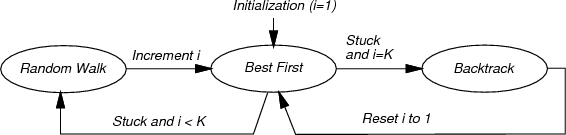
\includegraphics[width=1.0\linewidth]{images/planner.png}
		\caption{Randomized Potential Field Planner.}
		\label{RPP}
	\end{figure}
	
Más parámetros:

\begin{itemize}
\item Números de intentos del Best First.
\item Límite del Random Walk.
\item Número de Random Walks, $K$.
\end{itemize}
\end{frame}

\section{Trabajos Posteriores}

\begin{frame}{Gran Problema}{Desechado}
Debido a la gran cantidad de parámetros heurísticos que han de ajustarse para cada problema este tipo de algoritmos fueron \textbf{desechados} por otros que no emplean tantos parámetros.\\

\medskip

Aún así el método fue muy \textbf{influyente} en otros algoritmos de planificación basados en el muestreo. Aparecieron planificadores después del RPP que utilizaban también algún tipo de aleatoriedad en su algoritmo.
	
\end{frame}

\begin{frame}{Ariadne's Clew Algoritm}{Métodos Posteriores}

Destaca por tener dos modos de funcionamiento que se van alternando. En el modo \textbf{EXPLORE}, se añaden nuevos vértices de búsqueda en el mapa y en el modo \textbf{SEARCH}, se busca pasando por los vértices añadidos una ruta entre el punto inicial y el punto final libre de obstáculos.

\begin{itemize}
\item Mazer, Talbi, Ahuactzin and Bessière, 1992, \textit{The Ariadne's clew algorithm.}
\item Mazer, Ahuactzin and Bessière, 1998, \textit{The Ariadne's clew algorithm.}
\end{itemize}

\end{frame}

\begin{frame}{Expansive-space planner}{Métodos Posteriores}

Es similar al modo EXPLORE del algoritmo anterior, en donde se genera nuevos vértices en zonas menos visitadas del mapa. Además utiliza la búsqueda bidireccional para lograr una mayor eficiencia.

\begin{itemize}
\item Hsu, Latombe and Motwani, 1999, \textit{Path planning in expansive configuration spaces.}
\item Sánchez and Latombe, 2001, \textit{A single-query bi-directional probabilistic roadmap planner with lazy collision checking.}
\end{itemize}
\end{frame}

\begin{frame}{Random-walk planner}{Métodos Posteriores}

Se trata de un algoritmo eficiente que consiste en realizar movimientos aleatorios. Ajusta automáticamente los parámetros necesarios para cada movimiento basándose en los movimientos anteriores.

\begin{itemize}
	\item Carpin and Pillonetto, 2005, \textit{Merging the adaptive random walks planner with the randomized potential field planner.}
	\item Carpin and Pillonetto, 2005, \textit{Robot motion planning using adaptive random walks.}
\end{itemize}
\end{frame}

\begin{frame}{Rapidly Exploring Dense Trees}{Métodos Posteriores}

Este algoritmo es el más usado en la actualidad y se basa en la construcción de un árbol de configuraciones que crece explorando a partir de un punto origen. El árbol cubre uniformemente todo el espacio de configuraciones libres de colisión a través de dos pasos.

\begin{itemize}
	\item LaValle, 1998, \textit{Rapidly-exploring random trees: A new tool for path planning.}
	\item LaValle and Kuffner, 1999, \textit{Randomized kinodynamic planning.}
	\item LaValle and Kuffner, 2001, \textit{Rapidly-exploring random trees: Progress and prospects.}
\end{itemize}
\end{frame}

\begin{frame}{Roadmap Methods for múltiple queries}{Métodos Posteriores}

La finalidad de este algoritmo es construir un grafo topológico llamado roadmap, que eficientemente solucione múltiples peticiones iniciales. Las trayectorias en el roadmap deberían ser fácil de alcanzar para cada $q_I$ y $q_G$, y el grafo permita rápidas búsquedas de una solución.

\begin{itemize}
	\item Kavraki, Svestka, Latombe and Overmars, 1996, \textit{Probabilistic roadmaps for path planning in high-dimensional configuration spaces.}
\end{itemize}
\end{frame}

\begin{frame}
	\centering
	\LARGE{MUCHAS GRACIAS}\\
	\pause
	\bigskip
	\bigskip
	\Large{¿Preguntas?}
\end{frame}

\end{document}
